	%!TEX root = ../../Main.tex
\graphicspath{{Chapters/Krav/}}
%-------------------------------------------------------------------------------


\section{Krav}
I dette afsnit beskrives kravene til hvilken funktionalitet systemet har. 


I samarbejde med vejleder er der opstillet en række krav.
\begin{itemize}
\item Systemets skal kunne filtrere en støj fra et lydsignal, som indeholder et tale signal overlappet af et støjsignal.
\item Brugeren skal manuelt kunne tænde og slukke for filtreringen.
\item Lydsignalet skal feedes til en højtaler som afspiller lyden fra mikrofonen. 
\end{itemize}

Kravene er bygget op gennem use cases, som beskriver systemets funktionelle krav, samt en liste over alle ikke-funktionelle krav for systemet. Først vises aktørbeskrivelserne
med tilhørende aktørkontekst diagram. Herefter vises use cases for systemet. Der er udfærdiget to use cases
der tilsammen beskriver funktionaliteten af systemet. I use case afsnittet vises der også et use case diagram
med alle use cases og hvordan aktørerne interagerer med dem. Til sidst gives et kort overblik over ikke funktionelle krav.

\section{Aktørbeskrivelse}

\begin{figure}[H]
	\centering
	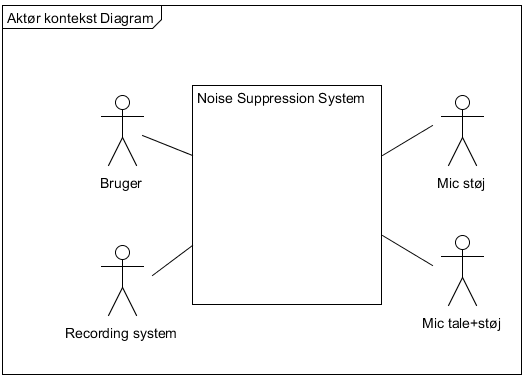
\includegraphics[width = 200 pt]{Img/Aktoer_Kontekst.png}
	\caption{Aktør Kontekst diagram}
	\label{fig:Aktoer Kontekst diagram}
\end{figure}

På figur \ref{fig:Aktoer Kontekst diagram} ses aktør kontekst diagrammet som beskriver sammenhængen mellem aktørene og det system de interagere med. Aktørene er som følger: \\*
\textbf{Primær}\\
\textbf{Bruger:} Den aktør der interagerer med systemet og vælger den ønskede funktionalitet \\
\textbf{Recording system:} Den aktør der modtager det enedelige produkt\\
\textbf{Sekundær}\\
\textbf{Mic støj:} Et input til det samlede system\\
\textbf{Mic tale+støj:} Et input til det samlede system \\

\section{Use case beskrivelse}

\begin{figure}[H]
	\centering
	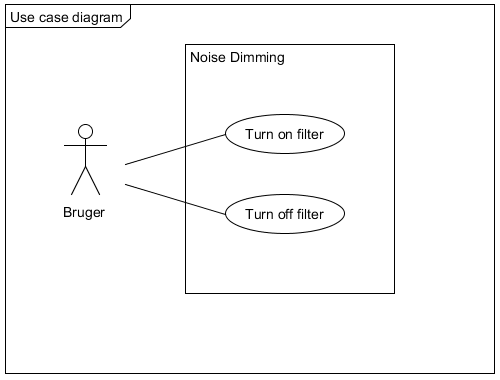
\includegraphics[width = 300 pt]{Img/Usecase_Diagram.png}
	\caption{Usecase diagram}
	\label{fig:Usecase diagram}
\end{figure}

På figur \ref{fig:Usecase diagram} ses usecase diagrammet som beskriver sammenhængen mellem aktørerne og de forskellige funktionaliteter der findes for systemet.

\subsubsection{UC 1 - Turn on filter}

Brugeren trykker på SW1 og filteret aktiveres. 


\subsubsection{UC 2 - Turn off filter}

Brugeren trykker på SW1 og filteret deaktiveres. 

\subsubsection{UC 3 - Filter aktiv}

Recording system modtager det filtrede lyd, hvis prækonditionen UC 1  er udført. 

\newpage
\section{Ikke-funktionelle krav}
Kravene er delt op i tre underkategorier. Krav der relaterer til problemet. krav der relaterer til DSP platform og algoritme. Til sidst er der en kategori der beskriver kravene til systemet på baggrund af de to første kategorier.
\begin{enumerate}
	
	\subsection{Problemrelateret krav}
	\item R1: Systemet skal have 2 mikrofoner og 1 højtaler
	
	\item R2: Filteret skal gøre brug af LMS algoritmen
	
	\item R3: Systemet skal kunne processerer lyd i frekvensbåndet 50-20000Hz. 
	
	\item R4: Systemet skal kunne dæmpe uønkset støj 30dB.
	
	\item R5: Systemet skal kunne dæmpe støj uden at dæmpe ønsket lydsignal.
	
	\item R6: Systemet burde have en latency under 30ms.
	
	\item R7: Systemet burde have et dynamikområde på min 96dB
	
	\subsection{System og algoritme krav}
	
	\item R8: Filter algoritmen skal implementeres med fixed point 
	
	\item R9: Filteret skal max bruge 10kByte memory
	
	\item R10: Filteret skal implementeres på Blackfin BF533
	
	\item R11: Filteret må max benytte 98\% DSP load

	\subsection{Afledte krav}
	
	\item DR1: DSP systemet skal kunne håndtere en samplingsrate på min 44100kHz(På baggrund af krav R3) 
	
	\item DR2: Filteret skal implementeres med 1.15 fixed point.(På baggrund af krav R7 og R8. Dette giver et dynamikområde på 96dB)
	
	\item DR3: Filter latency må max forsinkes 1280 samples(På baggrund af R6. (1/44100)*1280=30ms)
	
	\item Filteret må max bruge 13333 cycles af DSP processering for hver sample. 
	
\end{enumerate}


\section{Acceptest}
Til hver use case er der lavet en tilhørende accepttest, der tjekker om use casen bliver gennemført korrekt. Udover de tre accepttests er der oprettet en accepttest af de ikke-funktionelle krav til systemet. Alle accepttests kan ses
i kravspecifikations dokumentation.